\chapter{Background}
\label{background}


Using a case study we explore how network zoning is realized in modern enterprise networks, and later we derive the main challenges we confront.

\subsection{Case Study}
\label{ssec:casestudy}

Most enterprise networks have embraced the notion of layered security classification,
that can be broadly split into intranet, extranet, and opennet~\cite{ramasamy2011towards}. 
The opennet is the least trusted network (e.g., the Internet) which is an inhospitable region 
where live threats exist, whereas the intranet is the most trusted network hosting 
business-critical systems and sensitive information. Since the intranet has rigorous access 
control mechanisms to protect information assets from exposure to the opennet, enterprises are 
forced to operate another security layer (extranet, also known as demilitarized zone or DMZ) in between, which exposes the publicly 
accessible services to the opennet, while reducing the attack surface. 
% \ml{Is the extranet equivalent to the DMZ? If so, this term could already be introduced here.}

Over time, the layered network structure has become more sophisticated~\cite{obregon2015infrastructure}
due to extreme changes in network environments---diverse demands from customers, partners
and employees accessing enterprise networks with a variety of devices.
% As enterprises have recently witnessed extreme changes in network environment such as
% diverse demands from customers, partners and employees accessing their network with a
% variety of devices, enterprises employ more sophisticated network security 
% segmentation~\cite{obregon2015infrastructure}. 
% \claude{rephrase previous} 
As a result, many enterprise networks 
comprise a large number of zones defined by operational, organizational, and most
importantly security factors. Figure~\ref{fig:usecase} depicts a real-world use case for 
network zones running on inter-domain level with multiple involved autonomous systems (ASes). They 
can be categorized into three main types. 
% \ml{AS has not been introduced. Are people at NDSS generally familiar with the concept?}

\paragraph{Intra-domain Zone Transfer}
% 1. direct transfer
% 2. through trasit zone
Within a local network, multiple devices such as servers, databases, and hosts are connected
through network switches. These devices are assigned with a unique IP address that belongs
to a logically isolated network zone. These zones commonly consist of multiple subnets, 
often realized with a layer 2 virtualization technology (e.g., VLAN). Each zone is protected 
by a set of security middleboxes, e.g., firewalls, intrusion-prevention systems (IPS),
and intrusion-detection systems (IDS),
% \ml{IPS (intrusion-prevention system?) has not been introduced} 
which enforce predefined security policies for all traffic passing through.

To maintain the zone-based trust model, access permission to one zone is not considered to be 
valid for other zones. That is, an entity must obtain access permissions from all zones on the path when accessing a non-adjacent zone. This trust model
however often complicates policy management and enforcement, especially for large 
enterprise networks. 
% \claude{\sout{Consider a topology where three zones with different trust levels reside in a 
% linear arrangement, for example DMZ-Control-Database. If a Web server in the DMZ is 
% granted access to the Database zone but not the Control zone, firewalls in front of the 
% Control zone must be configured to distinguish packets coming from the Web server based 
% on the destination, and enforce different rules.}} 
To resolve this complication, the current practice introduces the notion of a dedicated zone transition
point, called Transit Zone.

A transit zone acts like a patch panel allowing zones to be interconnected without the need 
of a dedicated link between each pair of zones. The Transit zone sits in the middle of all 
the other zones and mediates access between zones wishing to communicate with each other.
% \claude{\sout{A Transit Zone is an attachment point that allows parallel connection of multiple zones.}}
It is commonly comprised of only forwarding devices (e.g., switches), interconnecting the 
attached zones via various ingress/egress points on which security middleboxes enforce the 
security policies. In a nutshell, the Transit Zone reduces the depth of zone hierarchies and 
thus simplifies the network zone design and management.

\begin{figure}[t]
\begin{center}
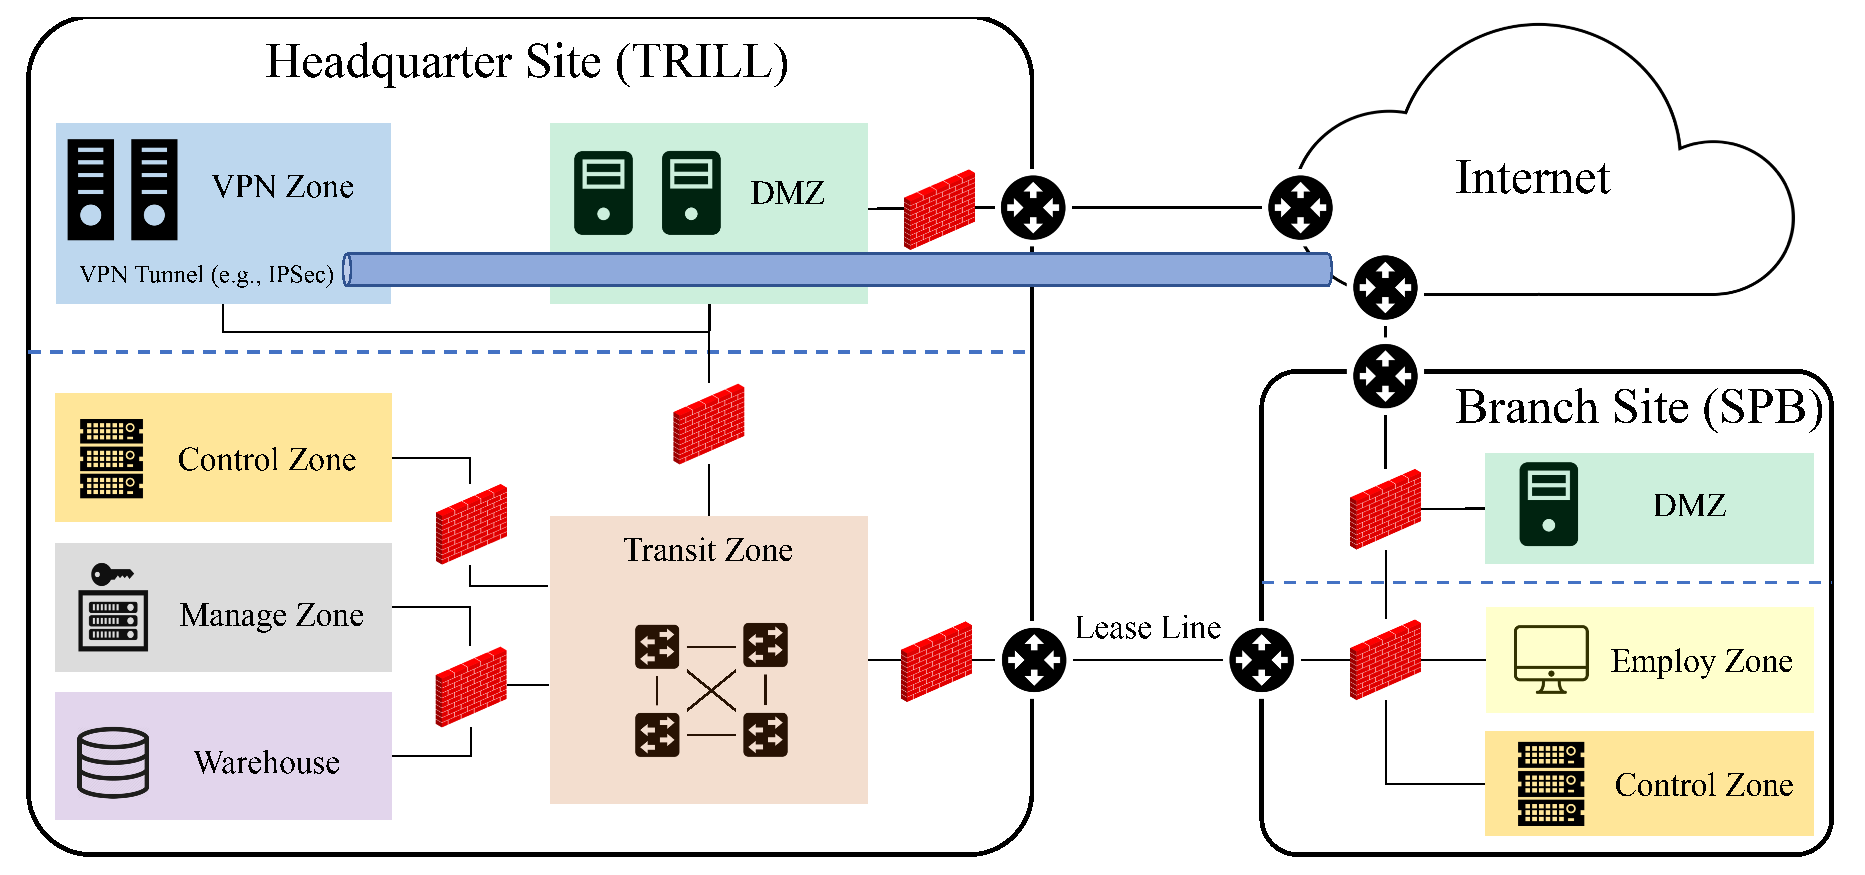
\includegraphics[width=.7\textwidth]{usecase.eps}
\end{center}
\caption{Network zoning use case for large enterprises. Network zones are 
realized with heavy use of security middleboxes (e.g., Firewalls).}
\label{fig:usecase}
\end{figure}

\paragraph{Inter-domain Zone Transfer}
% 1. to the same zone
% 2. to a different zone
To ensure that geographically distributed zones can securely communicate with each other, 
enterprises employ various networking technologies. The most common choice is connecting
two remote sites with a physical private line, (e.g., Layer 2 circuit). %or MPLS. 
% \ml{I would call an MPLS VPN a ``virtual private line'' as other traffic may flow over the same physical connections.} 
Enterprises 
can lease these lines from Internet service providers and make use of them to bridge local 
networks. However, purchasing private lines is costly and might come along 
with trust issues towards the service provider. 

An alternative is a virtual private 
network (VPN). A VPN uses cryptographic primitives to create a virtual tunnel between two 
local networks, preventing information leakage during transmission over the public Internet. 
While the VPN technology ensures data confidentiality, typically yet another layer of overlay 
protocols is required to achieve virtual separation of zones. The use of such overlay 
protocols, however, has the disadvantage that all interconnected sites need to deploy the same 
protocol since such protocols generally do not offer interoperability.

% \claude{While these techniques can be used to ensure confidentiality for data transmissions over an untrusted network, typically yet another layer of overlay protocols is required to achieve virtual separation of zones. The use of such overlay protocols, however, has the disadvantage that all interconnected sites need to deploy the same protocol since such protocols generally do not offer interoperability.}

% \claude{Where to put comparison of VPN point-to-point and \name Mondrian -> point to many}

\paragraph{Traffic from the Internet}
% 1. normal customer
% 2. authorised user (employ)
% 3. attacker
Traffic not originating from cooperative (trusted) networks can be classified 
into the following three types: i) public traffic, ii) authorized traffic, and iii) 
malicious traffic. The first case covers normal customers who access the enterprise's 
public services, e.g., Web servers. This traffic in general ends up at the demilitarized zone 
(DMZ) hosting only public services that require exposure to Internet. 
The second case refers to the traffic coming from temporarily authorized devices. For example,
a legitimate employee outside the enterprise's premises---working from home with a personal 
device---may get a temporal permit to access restricted zones via VPN. The last 
category comprises attack packets which are to be filtered by the security middleboxes in the frontline of defense.

% \begin{table}[t]
% % \caption{use case table. need to be merged with the fig_usecase}
% \label{tab:usecase}
% \centering
% \resizebox{0.48\textwidth}{!}{
% 	\begin{tabular}{*4{c}}
% 	\toprule
% 	& Between Zones & Through Transit Zone & Within Zone\\
% 	\midrule
% 	Inter-domain & \circled{1} $E_1 \leftrightarrow E_4$ 
% 	& \circled{2} $E_1 \leftrightarrow E_5$ & \circled{3} $E_1 \leftrightarrow E_2$\\
% 	Intra-domain & \circled{4} $E_5 \leftrightarrow E_6$ 
% 	& \circled{5} $E_3 \leftrightarrow E_4$ & \circled{6} $E_1 \leftrightarrow E_3$\\
% 	\bottomrule
% 	\end{tabular}
% }
% \end{table}

% \paragraph{Inter-domain Zone Transfer} % Case 1:
% \paragraph{Inter-domain Zone Transfer via Transit} % Case 2: 
% \paragraph{Inter-domain Communication within a Zone} % Case 3: 
% \paragraph{Local Zone Transfer} % Case 4: 
% \paragraph{Local Zone Transfer via Transit} % Case 5: 
% \paragraph{Local Communication within a Zone} % Case 6: 


\subsection{Challenges}
\label{ssec:challenges}

\paragraph{Secure Zone Transfer}
Transmitting security-sensitive data between zones in different physical locations (e.g., 
data center to branch site) over the public Internet poses a challenge. 
Security level information is lost in transit, requiring that the data is re-authenticated and 
filtered again on the receiving site even though source and destination could be part of the 
same logical zone.
Today's overlay protocols are often used to overcome the restriction of losing 
security level information in transit. This however introduces new challenges: difficulties 
in deployment per zone, computational overhead, and poor management scalability. 
% Driven by this, a light-weight zone transfer architecture is needed.

\paragraph{Interoperability}
Even if security-level information persists in transit, different zones might not be 
built on the same internal protocols (e.g., SPB~\cite{ieee2012spb} vs Trill~\cite{rfc6325}) 
which makes it difficult
for end systems in different zones to be able to seamlessly communicate with each other.
% A new architecture therefore must be able to understand various network protocols and 
% interpret them into a local language that all target networks can understand. This means 
% that the interpretation should preserve the properties of an original protocol, such as 
% % layer-2 routing decisions. 
% virtual segmentation.
% % A flexible design for the architecture to easily embed new protocols also should be considered.

\paragraph{Management Scalability}
In current local network zoning architectures, administration is being considered a tedious, 
time-consuming, and labor-intensive task. For example, simply adding a new zone might
require existing policies to be thoroughly reviewed, updated, and re-distributed
to the local network entities. The management complexity dramatically increases in a 
wide-area network (WAN) environment.
% For global orchestration across heterogeneous environments, a new architecture therefore
% must ensure management scalability. That is, network administrators should be able to easily extend 
% network zones in different physical locations and update policies that reflect these network
% changes, and be assured that no security loopholes were introduced.


% easily scale up resources 





% \subsection{Industrial Perspectives}

% % \paragraph{Large Enterprise Networks}
% % In order to protect information technology assets, large enterprise networks are partitioned into disjoint segments which group together assets with the same security requirements and policies. These groups are referred to as zones. Zones define the network boundaries and their defense requirements by stating the entities populating the zones, the entry points into the zone as well as how traffic is monitored and filtered at these entry points. Oftentimes, these zones are realized by a (virtualized) separation at layer 2 with firewalls at higher levels governing data transfers between zones.
% Traditionally, enterprises used to consider three security layers for their network 
% environment: intranet, extranet and opennet~\cite{ramasamy2011towards}. The opennet is
% the least trusted network (e.g., the Internet) which is inhospitable region where live 
% threats exist, while the intranet is the most trusted network hosting business-critical 
% systems and sensitive information. Since the intranet has rigorous access controls to 
% protect the information assets from an exposure, enterprises put another security layer 
% (extranet) in between, that only exposes public services to opennet and thus reduces 
% attack surfaces. 
% As enterprises have recently witnessed extreme changes in network environment such as
% diverse demands from customers, partners and employees accessing their network with
% variety of devices, the enterprises employ more sophisticated network security 
% segmentation\cite{obregon2015infrastructure}, called security zones.
% Security zones constitute the logical grouping of one or more subnets that share the
% same security requirements and policies. 
% % Since security zoning is the foundation of 
% % network isolation criteria that must be upheld for secure business environements, 
% % the zone classification of information assets requires 

% Each security zone is identified with different level of trust, and every pair of zones 
% are defined with a namely trusted-untrusted relationship. 
% To realize the unidirectional trust model, firewalls are considered as the most viable
% technologies and widely used in the current practice. However, operating firewalls in 
% large enterprises is often challenging to network operators and security architects. The 
% access control for the security zones might be dynamic, and thus its requires a complex 
% management scheme to accommodate a myriad set of policies. While there are advanced 
% technologies such as virtual firewall~\cite{deng2015vnguard,bakker2016network} and Unified
% Threat Management (UTM)~\cite{qi2007towards}, that are newly designed for enforcement of 
% access control polices in extremely dynamic networks, security zone management and modeling 
% still remains to be evolved~\cite{ramasamy2011towards,gontarczyk2015blueprint}.

% Bridging geographically distant security zones can also be challenging. Oftentimes,
% security zones are created not only for security purpose but also because of geographical
% factors. Given that the security zones in distance should exchange information over
% public network (opennet as aforementioned), there might be a potential risk that the
% communication may expose security-sensitive information during transit. To mitigate
% such a threat, network operators leverage additional security control/mechanisms (e.g.,
% IPSec~\cite{rfc4301} and SSL VPN~\cite{sun2011advantages}) which ensure confidentiality
% and integrity of the transmission over the untrusted network by encrypting the data with
% securely shared cryptographic keys. Nonetheless, the technologies might bring new challenges
% such as management scalability~\cite{felsch2018dangers} and compatibility to the secure 
% isolation~\cite{liu2008collaborative}.

% % \paragraph{Cloud Computing (LaaS, PaaS, SaaS)}
% The cloud computing environment is a good representative example that depicts such practical 
% challenges. Cloud-based service providers operate large multi-tenant data centers which 
% have to scale to customers needs. To achieve this scalability while at the same time staying
% cost efficient cloud providers make heavy use of virtualization techniques. This environment 
% challenges operators with providing secure segmentation between tenants as multiple tenants 
% are using the same physical machines and network. In addition, given that the cloud 
% environments comprise geographically distributed data centers, providing secure communication 
% channels between security zones while upholding a constant view of the security policies
% under the dynamic zone migration is another hill to climb. Now, we derive main challenges 
% we confront in this research with case study.
% % Legal requirements need to be respected. Furthermore, an optimal solution needs to be highly 
% % flexible as the number of assigned resources for a given customer can change frequently.



% % \paragraph{Edge Computing}
% % With the rise of mobile devices and Internet of Things (IoT) new types of data intensive, time sensitive applications are emerging. (e.g. VR/AR) However, since these devices are also required to be low power they cannot do these heavy computations themselves. Cloud computing can be used to offload the work to centralized data centers. However, this causes new challenges. Often, the latency between devices and the cloud is too high and therefore not well suited for real-time applications. Additionally, a large number of devices means that a centralized infrastructure can get saturated by big traffic flows. One widely used solution to this problem is Edge Computing which puts nodes handling the computation close to end devices.
